\chapter{RESULTS: GRAPHIC USER INTERFACE}
\label{chap:GUI_results.tex}
\addtocontents{toc}{\protect\setcounter{tocdepth}{1}}
The final GUI is a HTML page generated by the master {\it phyton} script which derives informations from assembly list files and execution log files. The generated .html file can be viewed by any standard web browser (like Internet Explorer, Firefox, Chrome) those support JavaScript. Care is taken that this htm is devoid of dependencies and hence enables interactive debug from remote locations. The only requirement for the user is network connectivity to receive the html page. The following figures shows various windows of final GUI
\section {EXECUTION FLOW GRAPH}
%\figurename{} 
\begin{figure}[h]
\centering
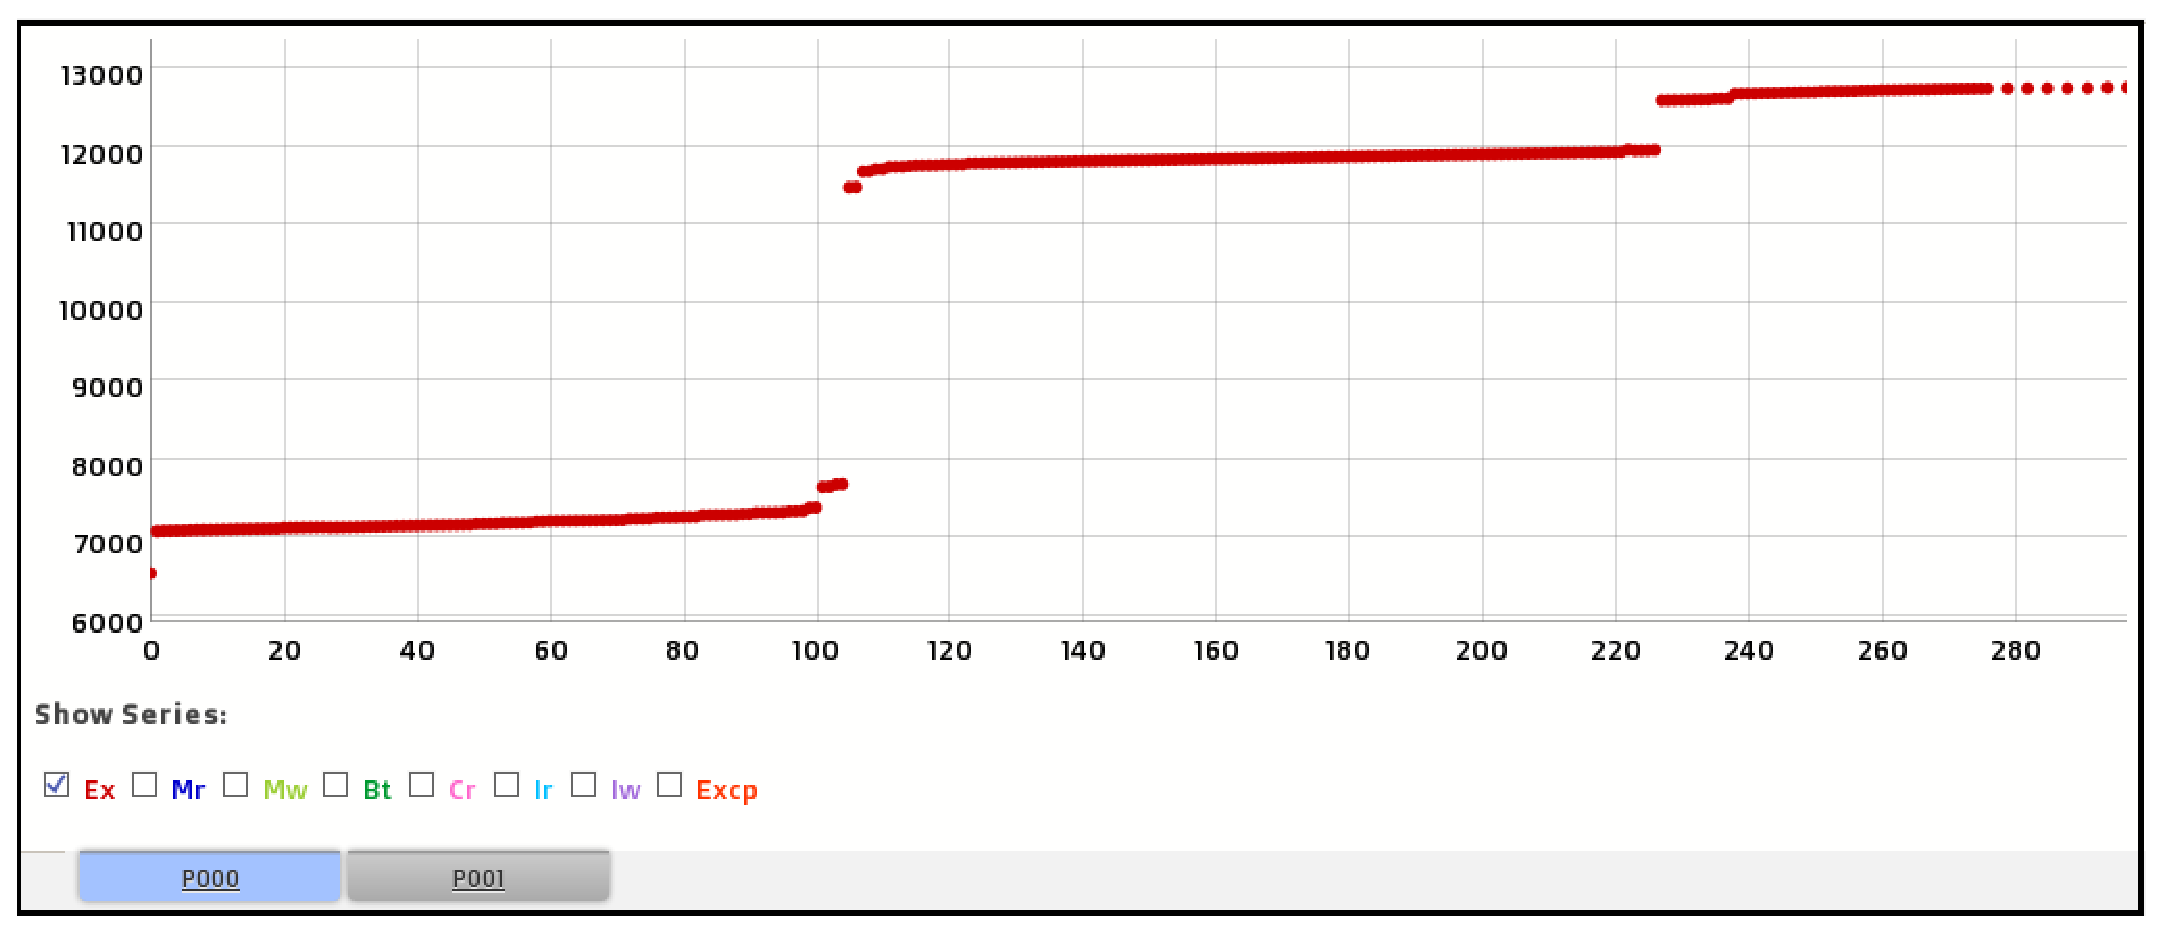
\includegraphics[width=6in]{./figures/gui_graph1.eps}
\caption{Execution Flow Graph}
\label{fig:gui_graph1.eps}
\end{figure}
%\end{tabular}
%\figurename{} 

~\figurename{~\ref{fig:gui_graph1.eps}}shows the main execution flow graph for selected active thread.  
\begin{figure}[h]
\centering
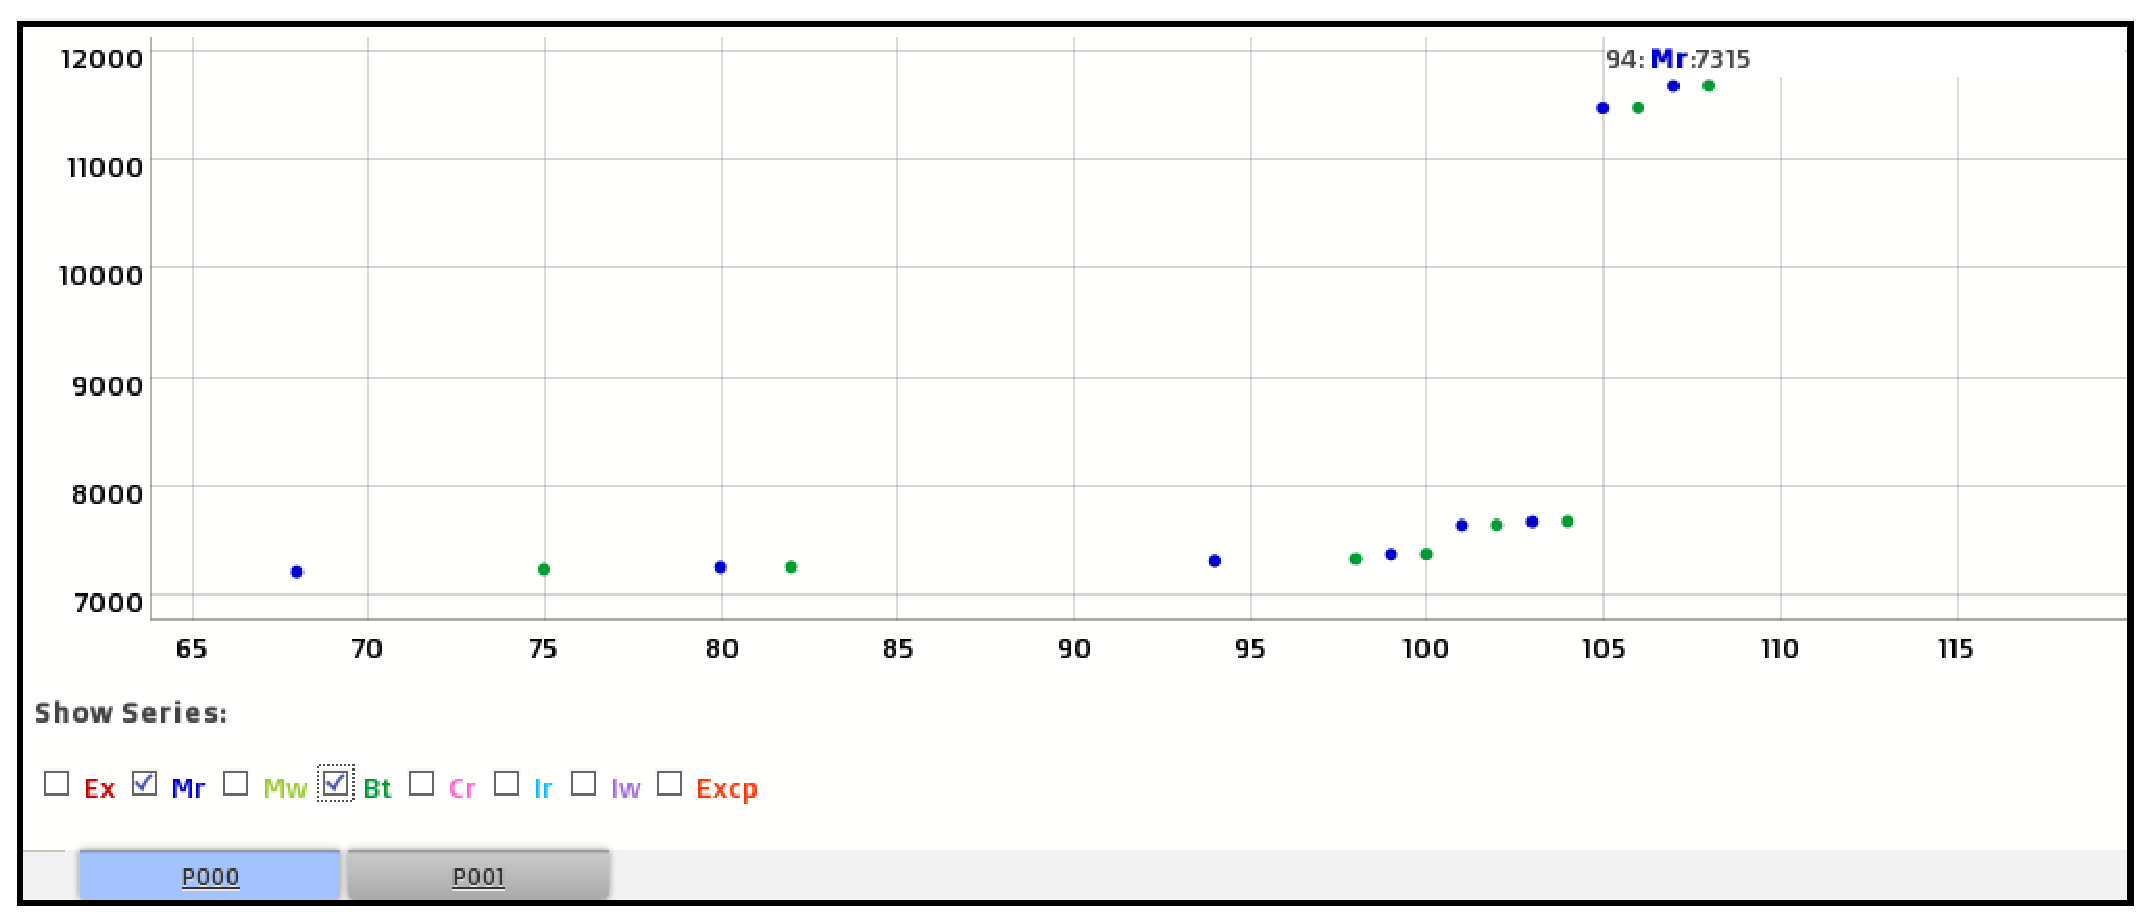
\includegraphics[width=6in]{./figures/gui_graph2.eps}
\caption{Execution Graph With Branching and Memory Writes}
\label{fig:gui_graph2.eps}
\end{figure}
%\end{tabular}
%\figurename{} 

~\figurename{~\ref{fig:gui_graph2.eps}} highlights execution points in which memory writes and branch operation occurs. The appropriate checkboxes towards bottom indicates the selection made. Note that thread {\it P000} is the active tab and inactive tab for {\it P001} is layered below it and could be selected.
\section {REGISTER WATCH WINDOW}
\begin{figure}[h]
\centering
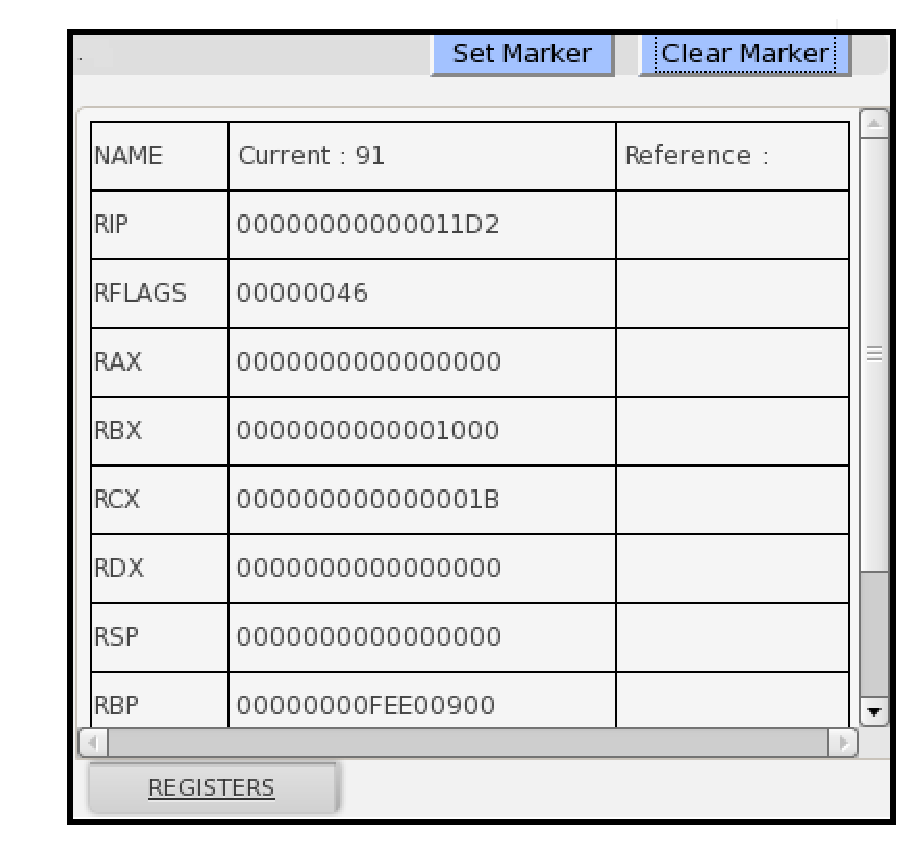
\includegraphics[width=4in, height=2in]{./figures/gui_reg1.eps}
\caption{Register Watch Window}
\label{fig:gui_reg1.eps}
\end{figure}
~\figurename{~\ref{fig:gui_reg1.eps}} is the register window. It could be observed that register values corresponding to selected execution point {\it cycle 91} is shown in {\it current selection} column. {\it Set~Marker} and {\it Clear~Marker} buttons could also be observed in the picture.
%\end{tabular}
\begin{figure}[h]
\centering
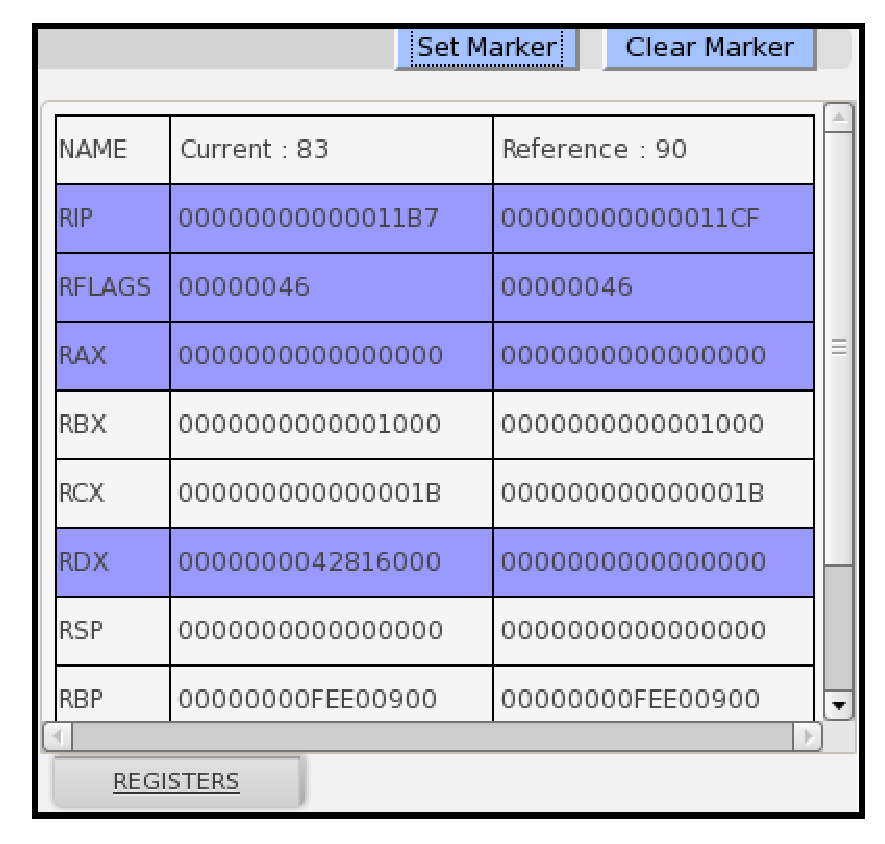
\includegraphics[width=4in, height=2in]{./figures/gui_reg2.eps}
\caption{Register Value Comparison}
\label{fig:gui_reg2.eps}
\end{figure}
%\end{tabular}
~\figurename{~\ref{fig:gui_reg2.eps}} shows the comparison of register states at two different points. Differences are highlighted.
\section {INSTRUCTION WINDOW}
\begin{figure}[h]
\centering
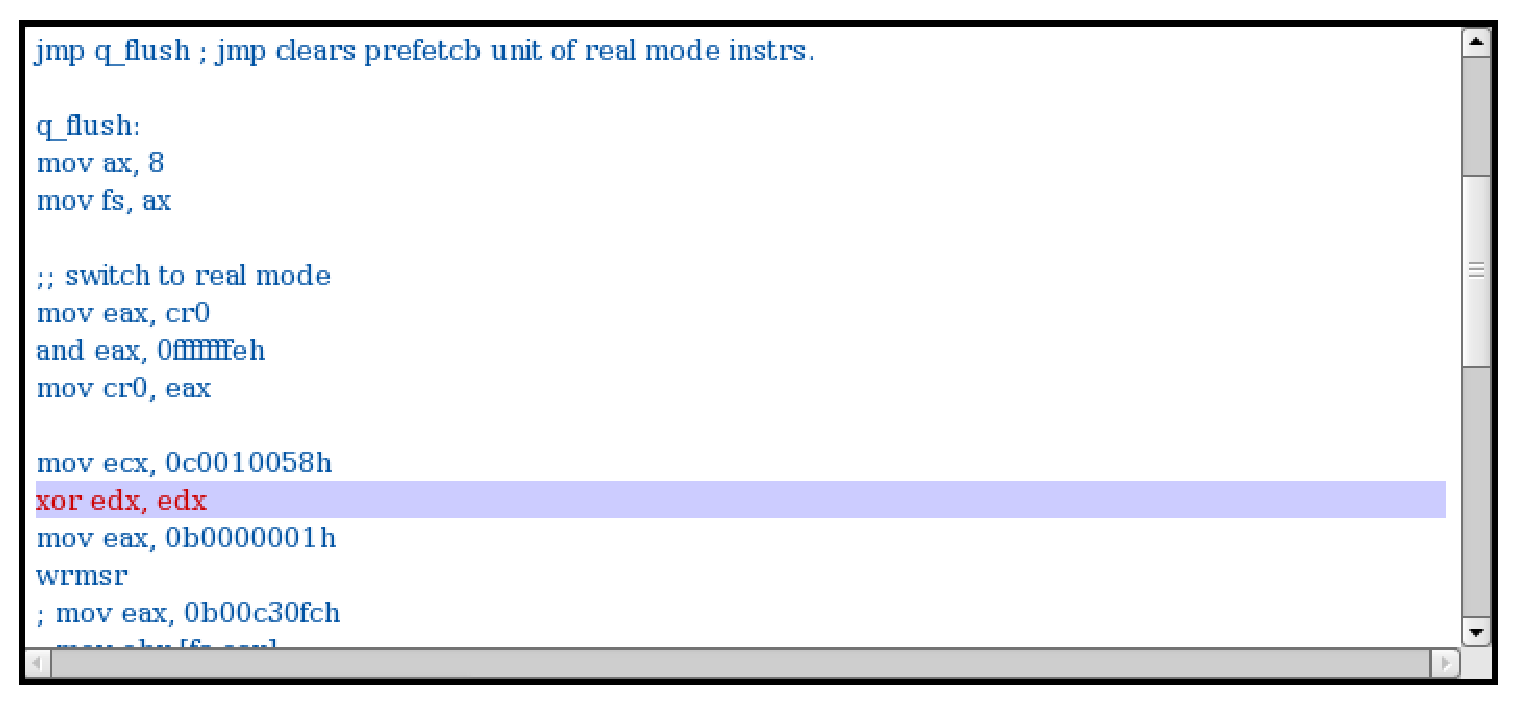
\includegraphics[width=5in, height=3in]{./figures/gui_asm.eps}
\caption{Instruction Window}
\label{fig:gui_asm.eps}
\end{figure}
%\end{tabular}
~\figurename{~\ref{fig:gui_asm.eps}} is the instruction window. The instruction window could be seen highlighting the assembly along with its context, corresponding to the selected execution point.


